\section{Processor Model}
\label{sec:methodology:processor_model}

\begin{figure}[ht]
\centering
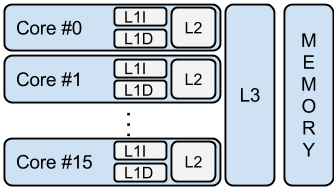
\includegraphics[scale=.65]{figures/processor_model/processor_model}
\caption{Processor model architecture}
\label{fig:processor_model}
\end{figure}

\begin{table}[ht]
\centering
\begin{tabular}{rl}
\toprule
\bf{Processor core}                 & 3GHz, OOO, 6 inst. dispatch width,     \\
                                    & 128 rob entries, 4 inst. commit width, \\
                                    & 3 Int. ALU, 1 FP MUL/DIV, 1 FP ADD, \\
                                    & 2 Int. SSE ALU, 1 Int. SSE MUL \\
\bf{Private L1 inst.}               & 32kB, 64B line-size, 4-way, 8 mshrs, LRU \\
\bf{Private L1 data}                & 32kB, 64B line-size, 8-way, 8 mshrs, LRU \\
\bf{Private L2 unified cache}       & 128/256/512/1024kB, 64B line-size, 8-way, \\
                                    & 12 MSHRs, LRU      \\
\bf{Shared L3 cache}                & 4/8/16/32MB, 64B line-size, 24 mshrs, \\
                                    & 32-way, varying replacement algorithm         \\
\bf{Memory controller}              & 6.4GB/s, 100ns access latency         \\
\bf{Clock Skew}                     & 100 cycle barrier synchronization        \\
\bottomrule                             
\end{tabular}
\caption{Model properties}
\label{tbl:processor_model:properties}
\end{table}

Throughout this thesis, we utilize a CMP model simulated on Sniper~\cite{Carlson2011a}. 
In our model, each processing core has two levels of private cache, the L1 data and code caches and a unified L2 cache.
Additionally there is a third cache level, L3, which is shared by all cores. 
The private caches are managed by an LRU replacement policy, and the replacement policy of the third cache level varies throughout our experiments.
Figure~\ref{fig:processor_model} shows an overview of the simulated architecture and Table~\ref{tbl:processor_model:properties} contains an overview of the system properties.

As the sniper simulation system implements a Nehalem core model, all our processor core properties are based on Intel's Nehalem architecture~\cite{Thomadakis2011}. 
The first level cache size is also selected based on the Nehalem architecture. 
We do note that in more recent architectures such as Intel's Haswell~\cite{Jain2013} the core properties have changed compared to the older Nehalem, but the size of the first level cache remains the same.
The reason being that with increasing cache size the access latency also increases. 
This in turn can cause problems if the first level cache is unable to feed the processor pipeline with a sufficient stream of instructions.

For our second cache layer, we have selected four different size configurations.
We will use these configurations to evaluate how cache partitioning algorithms running on the third cache level responds to changes in the size of private caches.
Our third level cache has three configurations.
During our experiment, we will choose a configuration based on the number of cores used.
For 4-, 8- and 16-core simulations we will respectively use a 4M, 8M, and 16M L3 configuration.

Snipers memory model is very limited compared to models in cycle-accurate simulators, such as gem5.
In our processor model each memory request completes in a constant 100ns, there is no simulation of row and column access delays.
Because inter-core interactions may be out-of-order, the memory bus model is a statistical model that attempts to estimate queuing delays based on a history window.
Both of these limitations introduces an error source in our simulations, but previous work~\cite{Carlson2011a, Olsen2014} has shown that results are still comparable to cycle-accurate simulations.
In order to reduce clock skewing caused by having multiple simulation threads, we utilize a 100 cycle barrier synchronization.
Barrier synchronization implies that all simulated cores must wait every 100 cycles for all other cores to catch up.
An experiment will be conducted to explore how big the effect on our results are when we change the synchronization period.

In the following sections, we describe how CACTI~\cite{Shivakumar2001} was used to estimate the access latency for each of our caches. 
When using CACTI we model each cache with parallel access to the tag directory and data.
We also opted for high-performance storage cells over the power saving ones that CACTI also supports.
Finally, we specify an optimization goal with a preference for lower access latencies.
To get a model that is as accurate as possible we have estimated the access latency for each configuration in both the L2 and the L3 caches.
As a result, we will correctly observe increasing access latencies with increasing cache sizes.


\subsection{L1 Code and Data Caches}

\begin{table}[ht]
\centering
\begin{tabular}{rrr}
\toprule
                          & \bf{Data}     & \bf{Instruction} \\
\bf{Size}                 & 32kB          & 32kB      \\
\bf{Block size}           & 64B           & 64B       \\
\bf{Associativity}        & 8             & 4         \\
\bf{Banks}                & 1             & 1         \\
\bf{Technology}           & 32nm          & 32nm      \\
\bf{Access time (Tag)}    & 0.16ns        & 0.16ns    \\
\bf{Access time (Data)}   & 0.38ns        & 0.32ns    \\
\bf{Access cycles (Tag)}  & 1             & 1         \\
\bf{Access cycles (Data)} & 2             & 1         \\
\bottomrule
\end{tabular}
\caption{L1 cache properties}
\label{tbl:processor_model:l1}
\end{table}

When choosing a first level cache size, we must consider that first level caches are on the critical path of the processor core.
Having a hit response latency of more than 2-3 cycles in a first level cache will be a limiting factor in the overall processor design.
We can observe that first level cache sizes have remained constant between Intel's Nehalem~\cite{Thomadakis2011} and the newer Haswell~\cite{Jain2013} architectures.
We have for this reason opted to simulate only a single size configuration at this cache level.
Both the first level caches have a size of 32kB; divided into sets of 4 and 8 lines for the instruction and data caches respectively. 
Both caches have 64-bytes long cache lines.
Table~\ref{tbl:processor_model:l1} summaries these values as well as the optimal bank count\footnote{We defined optimal bank count as the number of banks that provide the lowest access latency for data and tags measured in cycles.} and access latency for the tag directory and data as estimated by CACTI. 

We convert the access latency to cycles assuming a period of 0.3ns, equal to a clock speed of 3GHz.
For example, a tag access latency of 0.16ns equals one cycle while a data access latency of 0.38ns equals two cycles.
\subsection{L2 Cache}
\begin{table}[ht]
\centering
\begin{tabular}{rrrrr}
\toprule
\bf{Size}                 & 128kB       & 256kB       & 512kB       & 1024kB            \\
\bf{Block size}           & 64B         & 64B         & 64B         & 64B               \\
\bf{Associativity}        & 8           & 8           & 8           & 8                 \\
\bf{Banks}                & 1           & 2           & 8           & 8                 \\
\bf{Technology}           & 32nm        & 32nm        & 32nm        & 32nm              \\
\bf{Access time (Tag)}    & 0.28ns      & 0.29ns      & 0.26ns      & 0.32ns            \\
\bf{Access time (Data)}   & 0.57ns      & 0.66ns      & 0.88ns      & 0.95ns            \\
\bf{Access cycles (Tag)}  & 1           & 1           & 1           & 1                 \\
\bf{Access cycles (Data)} & 2           & 3           & 3           & 3                 \\
\bottomrule
\end{tabular}
\caption{L2 cache properties}
\label{tbl:processor_model:l2}
\end{table}

For the unified second level cache we have modelled four different sizes; 128kB, 256kB, 512kB and 1024kB. 
In all configurations, there are 8 lines in each set and each line is 64-bytes long.
Using CACTI, we have found the optimal number of banks per size configuration and the corresponding access latencies.
Table~\ref{tbl:processor_model:l2} summarises these values. 
Again we have converted access times to cycle assuming a 0.3ns period.
As expected we observe an access latency increase when the cache size increases.

\subsection{L3 Cache}
\begin{table}[ht]
\centering
\begin{tabular}{rrrrr}
\toprule
\bf{Size}                 & 4MB         & 8MB         & 16MB       \\
\bf{Block size}           & 64B         & 64B         & 64B         \\
\bf{Associativity}        & 32          & 32          & 32             \\
\bf{Banks}                & 4           & 4           & 4           \\
\bf{Technology}           & 32nm        & 32nm        & 32nm    \\
\bf{Access time (Tag)}    & 0.52ns      & 0.71ns      & 0.88ns   \\
\bf{Access time (Data)}   & 1.81ns      & 2.11ns      & 2.69ns     \\
\bf{Access cycles (Tag)}  & 2           & 3           & 3             \\
\bf{Access cycles (Data)} & 6           & 7           & 9      \\
\bottomrule
\end{tabular}
\caption{L3 cache properties}
\label{tbl:processor_model:l3}
\end{table}

Like the previous level we have three different size configurations for the L3 cache; 4MB, 8MB, and 16MB.
Unlike the previous two cache levels, that all use a standard LRU replacement policy, we will vary the replacement policy of the third level.
Many of the algorithms we are experimenting with in this work resemble some form of way-partitioning by assigning a number of ways (or cache lines) per cache set to each core.
For this reason, the third level cache has 32 cache lines per cache set, in contrast to the 16 cache lines per set in the original Nehalem architecture.
Giving us an average of 8/4/2 sets per core during our 4/8/16 core experiments.
The line size is set to be 64-bytes as in the previous level.
Again using CACTI we find the optimal bank count and the corresponding access latencies.
Table~\ref{tbl:processor_model:l3} summarises the cache properties for the various cache sizes.